In the diagram below, $P, Q, R$ are points on $BC, CA, AB$ respectively such
that the lines $AP, BQ, CR$ are concurrent at $X$. Also $PR$ bisects $\angle
BRC$, i.e. $\angle BRP = \angle PRC$. Prove that $\angle PRQ = 90^{\circ}$.

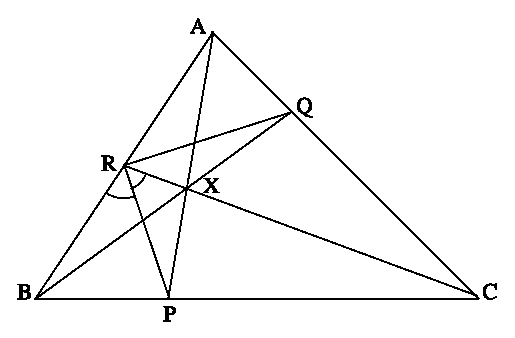
\includegraphics{vtrmc-2007-problem4.eps}
